\documentclass{bredelebeamer}
\usepackage{amsfonts}
\usepackage{amsmath}
\usepackage{multirow}
\usepackage{bbm}
\usepackage{xparse}

%% OPTIONS

\graphicspath{{./images/}}
\def\bc{\begin{center}}
	\def\ec{\end{center}}
%========================================================
\def\bit{\begin{itemize}}
	\def\eit{\end{itemize}}

\def\la{{\langle}}
\def\ra{{\rangle}}
\def\da{\,{\partial_a}}


\def\ind{{\bf 1}}
\def\demi{\frac{1}{2}}

\AtBeginSection[]{
	\begin{frame}
		\vfill
		\centering
		\begin{beamercolorbox}[sep=8pt,center,shadow=true,rounded=true]{title}
			\usebeamerfont{title}\insertsectionhead\par%
		\end{beamercolorbox}
		\vfill
	\end{frame}
}

\newenvironment<>{varblock}[2][.9\textwidth]{%
	\setlength{\textwidth}{#1}
	\begin{actionenv}#3%
		\def\insertblocktitle{#2}%
		\par%
		\usebeamertemplate{block begin}}
	{\par%
		\usebeamertemplate{block end}%
\end{actionenv}}


\def\t{{\texttt{t}}}
\def\logit{\,{\text{logit}}\,}
\def\x{\times}
\def\ox{\otimes}
\def\ind{{\bf 1}}
\def\demi{\frac{1}{2}}
\def\d{\text{d}}
\def\cvlaw{\,{\buildrel law \over \rightarrow}\,}

\def\eqd{\,{\buildrel d \over =}\,}
\def\cvweak{\,{\buildrel weak \over \rightarrow}\,}
\def\cvvague{\,{\buildrel vague \over \rightarrow}\,}
\def\A{{\mathcal{A}}}
\def\E{{\mathbb{E}}}
\def\R{{\mathbb{R}}}
\def\H{{\mathbb{H}}}
\def\P{{\mathbb{P}}}
\def\Q{{\mathbb{Q}}}
\def\N{{\mathbb{N}}}
\def\tX{{\tilde{\mathcal{X}}}}
\def\1{{\mathbf{1}}}
\def\ind{{\mathbf{1}}}
\def\F{{\mathcal{F}}}
\def\G{{\mathcal{G}}}
\def\M{{\mathcal{M}}}
\def\MP{{\mathcal{M}_P}}
\def\X{{\mathcal{X}}}
\def\tX{{\tilde{\mathcal{X}}}}
\def\Y{{\mathcal{Y}}}
\def\logit{{\text{logit}}}
\def\d{{\mathrm{d}}}
\def\D{{\mathbb{D}}}
\def\C{{\mathbb{C}}}
\def\H{{\mathcal{H}}}
\def\tGamma{{\tilde{\Gamma}}}
\def\tQ{{\tilde{Q}}}
\def\blambda{{\bar{\lambda}}}
\def\bb{{\bar{b}}}
\def\bd{{\bar{d}}}
\def\be{{\bar{e}}}
\def\bk{{\bar{k}}}
\def\ba{{\bar{a}}}
\def\bxi{{\bar{\xi}}}
\def\bl{{\bar{l}}}
\def\la{{\langle}}
\def\ra{{\rangle}}
\def\tN{{\tilde{N}}}
\def\bN{{\bar{N}}}
\def\bZ{{\bar{Z}}}
\def\ttau{{\tilde{\tau}}}
\def\btau{{\bar{\tau}}}
\def\bX{{\bar{X}}}
\def\bm{{\bar{m}}}
\def\bC{{\bar{C}}}
\def\bD{{\bar{D}}}
\def\bA{{\bar{A}}}
\def\bJ{{\bar{J}}}
\def\bu{{\bar{u}}}
\def\bv{{\bar{v}}}


\def\tg{{\tilde{g}}}
\def\tb{{\tilde{b}}}
\def\td{{\tilde{d}}}
\def\te{{\tilde{e}}}
\def\tk{{\tilde{k}}}

\def\Var{{\mathrm{Var}}}
\def\Cov{{\mathrm{Cov}}}

\def\Var{{\mathrm{Var}}}
\def\Cov{{\mathrm{Cov}}}
\def\CV{{\mathrm{CV}}}
\def\Corr{{\mathrm{Corr}}}

\def\bT{{\bar{T}}}


\def\du{\,{\partial_u}}
\def\da{\,{\partial_a}}
\def\ds{\,{\partial_s}}
\def\dt{\,{\partial_t}}
\def\dn{\,{\partial_n}}
\def\txi{{\tilde{\xi}}}

%\def\bmu{{\bar{\mu}}}
\def\bmu{{\mu}}

\def\dlambda{\,{\partial_\lambda}}
\def\dlambdak{\,{\partial_{y_k}}}
\def\dmu{\,{\partial_\mu}}
\def\dn{\,{\partial_n}}
\def\txi{{\tilde{\xi}}}
\def\tr{{\text{Tr}}}

\def\cblue{{\color{titleColor}}}

\def\cbrun{{\color{alertTitleBlockColor}}}

%%%%%%%%%%%%%%%%%%%%%%%

\title[]{Latent Space Oddity On The Curvature Of Deep Generative Models}
% Titre du diaporama

%\subtitle{}
% Sous-titre optionnel

\author{Clément \textsc{Gris}i, Timothée \textsc{Darcet}}
% La commande \inst{...} Permet d'afficher l' affiliation de l'intervenant.
% Si il y a plusieurs intervenants: Marcel Dupont\inst{1}, Roger Durand\inst{2}
% Il suffit alors d'ajouter un autre institut sur le modèle ci-dessous.

\institute[ENS Paris-Saclay]

\date{6 janvier 2020}
% Optionnel. La date, généralement celle du jour de la conférence

\subject{Sujet de votre diaporama}
% C'est utilisé dans les métadonnes du PDF

\logo{}

%%%%%%%%%%%%%%%%%%%%%%%%%%%%%%%%%%%%%%%%%%%%%%%%%%%%%%%%%%%%%%%%%%%%%
\begin{document}
	
	\begin{frame}
		\titlepage
	\end{frame}
	
	\section{Generative Models}
	
	\begin{frame}
		\frametitle{Goal}
		
		Given training data, generate new samples from the same distribution
		
		\begin{figure}
			\centering
			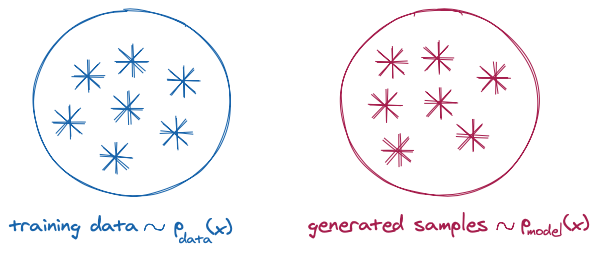
\includegraphics[scale=0.3]{../fig/density_estimation.png}
		\end{figure}
		
		\begin{center}
			\begin{minipage}{5cm}
				\begin{varblock}[5cm]{}
					\centering
					learn $p_{\text{model}}(x)$ close to $p_{\text{data}}(x)$
				\end{varblock}
			\end{minipage}
		\end{center}
		
	\end{frame}
	
	\begin{frame}
		\frametitle{Density estimation}
		
		\bit
		\item core problem in the \textbf{unsupervised} learning setting
		\item explicit: explicitly define and solve $p_{\text{model}}(x)$ 
		\item implicit: learn a model that can sample from $p_{\text{model}}(x)$ without explicitly defining it
		\eit
		
		%goal: learn some underlying hidden \textbf{structure} of the data \\
		%$\rightarrow$ \textit{clustering, dimensionality reduction, density estimation}
		
	\end{frame}
	
	\section{Variational Auto Encoders}
	
	\begin{frame}
		\frametitle{Auto encoders}
		
		unsupervised approach for learning a lower dimensional feature representation \textbf{z} from unlabeled training data $x$
		
		\begin{figure}
			\centering
			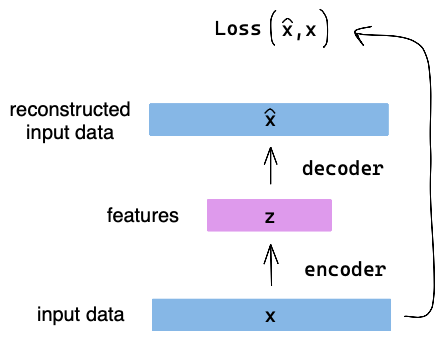
\includegraphics[scale=0.3]{../fig/ae.png}
		\end{figure}
		
		\textbf{z} captures meaningful factors of variation in the data\\
		
		\vspace{3mm}
		\centering
		\textbf{Question: can we generate new images from an auto encoder?}
		
	\end{frame}
	
	\begin{frame}{Variational auto encoders}
		
VAEs are a probabilistic spin on auto encoders that will let us sample from the model to generate data\\

\vspace{2mm}

Assumption: training data $\{ x_i \}_{i \in [1,N]}$ is generated from underlying (latent) \textbf{unobserved} representation \textbf{z}\\

\vspace{2mm}

\begin{figure}
	\centering
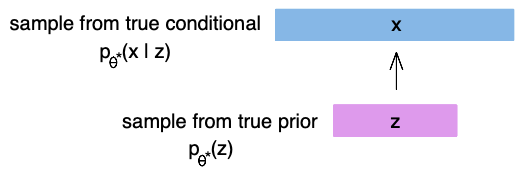
\includegraphics[width=5cm]{../fig/x_from_z.png}
\end{figure}

\textbf{Goal:} estimate the true parameters $\theta^*$ of this generative model\\

\vspace{3mm}
\centering
\textbf{Question: how do we train the model?}
		
\end{frame}
	
\begin{frame}{Intractability}
Choose simple prior $p(z)$ (e.g. Gaussian)\\
Conditional $p(x \vert z)$ is \textbf{complex}: represent it with a neural network\\
\vspace{3mm}
Natural strategy: learn model parameters to maximize the likelihood of the training data
	
	\begin{align*}
		p_{\theta}(x) = \int p_{\theta}(x \vert \textbf{z}) p_{\theta}(\textbf{z}) d\textbf{z}
	\end{align*}
	
	Though we know $p_{\theta}(x \vert \textbf{z})$ and $p_{\theta}(\textbf{z})$, it is \textbf{intractable} to compute $p_{\theta}(x \vert \textbf{z})$ for every $z$!\\
	
	\vspace{3mm}
	
	Posterior density is also \textbf{intractable}: 
	
	\begin{align*}
		p_{\theta}(\textbf{z} \vert x) = \dfrac{p_{\theta}(x \vert \textbf{z}) p_{\theta}(\textbf{z})}{p_{\theta}(x)} 
	\end{align*}
	
\end{frame}

\begin{frame}
	\frametitle{Solution}
	
	In addition to the \textbf{decoder} network modeling $p_{\theta}(x \vert z)$, define an additional \textbf{encoder} network $q_{\delta}(z \vert x)$ that approximates  $p_{\theta}(z \vert x)$.\\
	
	\begin{figure}
		\centering
		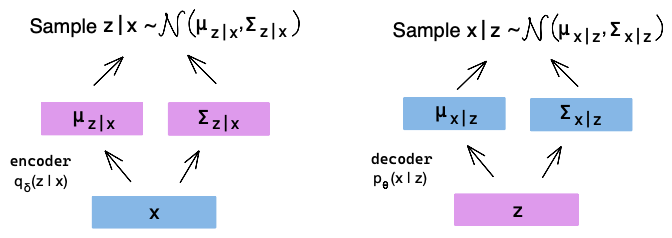
\includegraphics[scale=0.4]{../fig/p_and_q.png}
	\end{figure}
	
	
	This allows us to derive a \textbf{tractable} lower bound on the data likelihood
	
\end{frame}


\begin{frame} 
	\frametitle{Tractable lower bound}
	
	\begin{align*}
		\log p_{\theta}(x) & = \mathbb{E}_{z \sim q_\delta(\cdot \vert x)} \big[ \log p_{\theta}(x) \big]\\
		& = \mathbb{E}_{z} \left[ \log \dfrac{p_{\theta}(x \vert z)p_{\theta}(z)}{p_{\theta}(z \vert x)} \right]\\
		& = \mathbb{E}_{z} \left[ \log \dfrac{p_{\theta}(x \vert z)p_{\theta}(z)}{p_{\theta}(z \vert x)} \dfrac{q_\delta(z \vert x)}{q_\delta(z \vert x)} \right]\\
		& = \mathbb{E}_{z} \left[ \log p_{\theta}(x \vert z) \right] - \mathbb{E}_{z} \left[ \log \dfrac{q_\delta(z \vert x)}{p_{\theta}(z)} \right] + \mathbb{E}_{z} \left[ \log \dfrac{q_\delta(z \vert x)}{p_{\theta}(z \vert x)} \right] \\
		& = \textcolor{Framavert}{ \mathbb{E}_{z} \left[ \log p_{\theta}(x \vert z) \right]} - \textcolor{Framableu}{d_{\text{KL}} \left( q_\delta(z \vert x) \vert \vert p_{\theta}(z) \right)} + \textcolor{Framaorange}{ d_{\text{KL}} \left( q_\delta(z \vert x) \vert \vert p_{\theta}(z \vert x) \right)} \\
	\end{align*}
	
\end{frame}

\begin{frame}
	\frametitle{Tractable lower bound}
	
	- decoder network gives $p_\theta(x \vert z)$: we can estimate $\textcolor{Framavert}{ \mathbb{E}_{z} \left[ \log p_{\theta}(x \vert z) \right]}$ through sampling (differentiable with the reparametrization trick)\\
	- $\textcolor{Framableu}{d_{\text{KL}} \left( q_\delta(z \vert x) \vert \vert p_{\theta}(z) \right)}$ is the KL-div of two Gaussian distributions: it has a nice closed from solution (differentiable)\\
	- though $p_\theta(z \vert x)$ is intractable, we know KL-div is always positive: $\textcolor{Framaorange}{ d_{\text{KL}} \left( q_\delta(z \vert x) \vert \vert p_{\theta}(z \vert x) \right)} \geq 0$\\
	
	\vspace{5mm}
	
	Hence,
	
	\begin{align*}
		\log p_{\theta}(x) & \geq \textcolor{magenta}{ \mathbb{E}_{z} \left[ \log p_{\theta}(x \vert z) \right] - d_{\text{KL}} \left( q_\delta(z \vert x) \vert \vert p_{\theta}(z) \right) }\\
		& \geq \textcolor{magenta}{\mathcal{L} (x, \theta, \delta)}
	\end{align*}
	
	We've identified a \textbf{tractable} + \textbf{differentiable} lower bound which we can take gradient of and optimize (ELBO, evidence lower bound)
	
\end{frame}

\begin{frame}
	\frametitle{Training}
	
	Optimal parameters will be the ones that maximize this lower bound: 
	
	\begin{align*}
		\theta^*, \delta^* = \arg \max_{\theta, \delta} \sum_{i=1}^{N} \mathcal{L} (x_i, \theta, \delta)
	\end{align*} 

	In order to find them with stochastic gradient descent, we need to compute and backpropagate $\nabla_\theta \mathcal{L} \left(\theta, \delta \right)$ and $\nabla_\delta \mathcal{L} \left(\theta, \delta \right)$.\\
	
	\vspace{3mm}
	
	Computing $\nabla_\theta \mathcal{L} \left(x_i, \theta, \delta \right)$ for a given input data $x_i$ is relatively straightforward. However, computing $\nabla_\delta \mathcal{L} \left(x_i, \theta, \delta \right)$ is harder as the parameter $\textcolor{magenta}{\delta}$ appears in the distribution with respect to which the expectation $\mathbb{E}_{z \sim q_{\textcolor{magenta}{\delta}}(\cdot \vert x_i)} \left[ \log p_\theta(x_i \vert z)\right]$ is taken:
	
	\begin{equation*}
		\begin{aligned}
			\nabla_{\textcolor{magenta}{\delta}} \mathbb{E}_{z \sim q_{\textcolor{magenta}{\delta}}(\cdot \vert x_i)} \left[ \log p_\theta(x_i \vert z)\right] \quad \neq \quad \mathbb{E}_{z \sim q_{\textcolor{magenta}{\delta}}(\cdot \vert x_i)} \left[ \nabla_{\textcolor{magenta}{\delta}} \log p_\theta(x_i \vert z)\right]
		\end{aligned}
	\end{equation*}
	
\end{frame}

\begin{frame}
	\frametitle{Reparametrization trick}
	
	Our goal is to rewrite this expectation in such a way that $\delta$ appears inside the expectation only:
	
	\begin{equation*}
		\begin{aligned}
			\mathbb{E}_{z \sim q_{\textcolor{magenta}{\delta}}(\cdot \vert x_i)} \left[ \log p_\theta(x_i \vert z)\right]= \mathbb{E}_{p_\varepsilon} \left[ \log p_\theta \left(x_i \vert g_{\textcolor{magenta}{\delta}}(\varepsilon, x_i) \right) \right]
		\end{aligned}
	\end{equation*}
	
	\vspace{1mm}
	
	such that $g_{\textcolor{magenta}{\delta}}(\varepsilon, x_i)  = z \sim \mathcal{N} \left(\mu_{z \vert x_i}, \Sigma_{z \vert x_i}\right)$
	
	\vspace{3mm}
	
	We can sample from $\mathcal{N} \left(\mu_{z \vert x_i}, \Sigma_{z \vert x_i}\right)$ by first sampling $\varepsilon \sim \mathcal{N} \left(0, 1\right)$ and computing:
	
	\begin{equation*}
		\begin{aligned}
			z = g_{\delta}(\varepsilon, x_i)  = \mu_{z \vert x_i} + \left( \Sigma_{z \vert x_i}\right)^{\frac{1}{2}} \varepsilon
		\end{aligned}
	\end{equation*}
	
	This function $g$ is a simple linear transform (deterministic) and allows us to compute $\nabla_\phi \textbf{L}\left(\theta, \phi \right)$.

\end{frame}

\begin{frame}
	\frametitle{Training}
	
	\begin{figure}
		\centering
		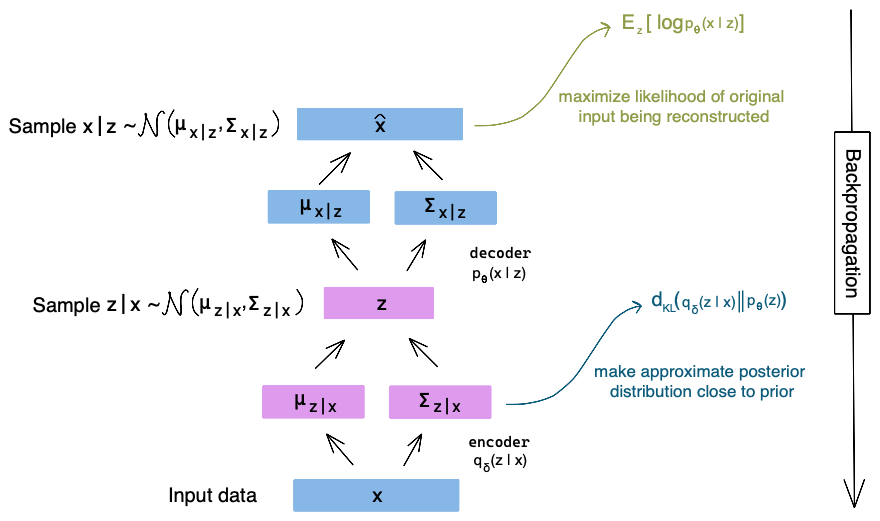
\includegraphics[scale=0.33]{../fig/vae.png}
	\end{figure}
	
\end{frame}

\begin{frame}
\frametitle{Data generation}

Once trained, we can sample \textbf{z} from prior and use the decoder network to generate new data:

\begin{figure}
	\centering
	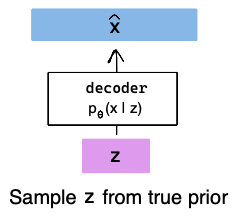
\includegraphics[scale=0.4]{../fig/generate_data.png}
\end{figure}

\end{frame}

\section{Latent Space Oddity}

\begin{frame}
\frametitle{A misinterpretation of the latent space}

\textbf{Goal:} equiped with a good latent space, points from the same class should be clother to each other than to members of the other classes

\vspace{3mm}

\begin{figure}
	\centering
	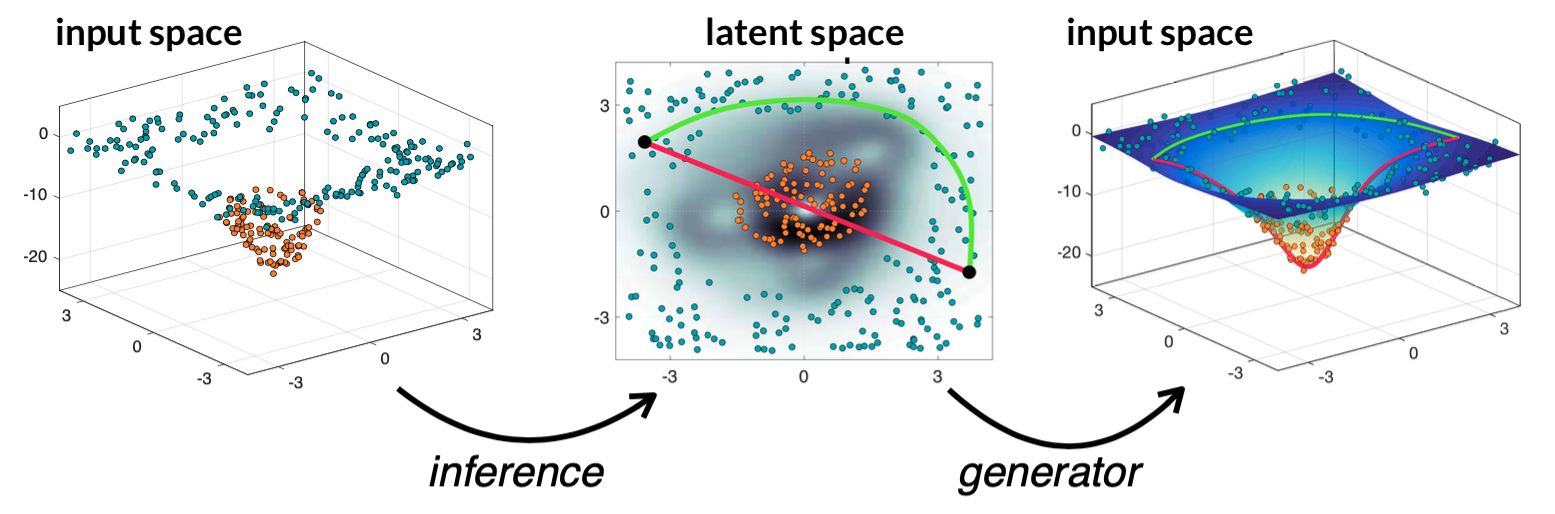
\includegraphics[width=10cm]{../fig/input_to_latent_to_input.png}
\end{figure}

\textbf{Issue:} this doesn't \textit{seem} to be the case (\textcolor{green}{green} path is actually shorter than \textcolor{red}{red} path)\\

\end{frame}

\begin{frame}
	
fThis \textit{seemed} conclusion is incorrect\\
$\rightarrow$ this is due to a misinterpretation of the latent space: it shouldn't be seen as a linear Euclidian space but rather as a \textbf{curved} space\\

\vspace{3mm}
\begin{block}{} 
This curvature induces a Riemannian metric which gives more meaningful distances than the usual Eulidian distance
\end{block}

% implies that the natural interpolant between two latent points is no longer a straight line, but a curve

\end{frame}

\section{Geometry of the decoder}

\begin{frame}
	\frametitle{VAE decoder}
	
The decoder driving VAEs is \textbf{stochastic}:

\begin{align*}
	f(z)= \mu(z) + \sigma(z)  \odot \varepsilon \quad  \left( \varepsilon \sim \mathcal{N}(0, \mathbb{I}_D) \right)
\end{align*} 

$\rightarrow$ this implies a \textbf{stochastic} Riemannian geometry

\vspace{2mm}
\begin{block}{Theorem 1} 
	if stochastic decoder is at least twice differentiable, the expected metric equals:
	\begin{align*}
		\overline{\text{M}}_z = \mathbb{E}_{p(\varepsilon)} \left[ \text{M}_z\right] = \left( \text{J}_z^{(\mu)} \right)^\top \left( \text{J}_z^{(\mu)} \right) + \left( \text{J}_z^{(\sigma)} \right)^\top \left( \text{J}_z^{(\sigma)} \right)
	\end{align*} 
\end{block}
\vspace{2mm}
where $\text{J}_z^{(\mu)}$ and $\text{J}_z^{(\sigma)}$ are the jacobian matrices of $\mu(\cdot)$ and $\sigma(\cdot)$

\end{frame}

\begin{frame}
\frametitle{VAE decoder}
	
Coupled with Theorem 2, we get that the (deterministic) expected metric $\overline{\text{M}}_z$ is a good approximation to $\text{M}_z$ when the data dimension is large: we can use the theory of deterministic decoders

\vspace{2mm}
\begin{block}{Theorem 2} 
	\centering
	$\lim_{D \rightarrow \infty} \text{Var} \left( \text{M}_z \right) = 0$
\end{block}
\vspace{2mm}

The resulting induced distance will be large in regions of the latent space where the decoder is highly uncertain (high variance)\\
$\rightarrow$ shortest paths will tend to avoid these regions

\end{frame}

\begin{frame}
\frametitle{Ensuring proper geometry}

The geometry of a VAE depends on both the mean and the variance of its decoder\\
$\rightarrow$ successful training will provide good estimates of the geometry in regions near the data\\

\vspace{3mm}

The decoder is expected to have high variance in regions with no data\\
In practice, variance estimates are extrpolated to regions without data: as neural nets extrapolate poorly, practical variance estimates tend to be poor in regions with no data...\\

\vspace{3mm}

\textbf{Issue:} we need well-behaved variance functions to ensure a well-behaved geometry
	
\end{frame}

\begin{frame}
\frametitle{Regularizing the geometry}

\textbf{Solution:} model decoder's \textit{precision} instead of its variance\\

\vspace{3mm}

\textbf{add more details}

\vspace{3mm}

The measure element: $\sqrt{\text{det}\left(\text{M}_z\right)}$\\

\vspace{3mm}

\textbf{add more details}

\vspace{3mm}

In constrast to the standard model, the proposed model provides a clear geometrical structure that follows the trend of the data
\end{frame}

\begin{frame}
\frametitle{Conclusion}

\bit
\item standard model assigns \textcolor{Framarouge}{arbitrary} density in regions of the input space where data has not been seen during training, while the proposed model assigns \textcolor{Framavert}{minimal density} to such regions
\item the variance term of the standard model behaves \textcolor{Framarouge}{arbitrarily} in regions with no latent codes, whereas the proposed model assigns \textcolor{Framavert}{high variance} in those regions
\eit

\vspace{3mm}

\textbf{Result:} proposed model achieves better marginal likelihood on held-out data

\end{frame}

\section{Experiments}

\begin{frame}
	\frametitle{Experiments}
	

\end{frame}

\begin{frame}
	Bibliography :
	
	\vspace{2mm}
	
	\nocite{*}
	\small{\bibliographystyle{unsrt}
		\bibliography{biblio}\vspace{0.75in}}
	
\end{frame}

\end{document}